\subsection*{Additional appendices}
\phantomsection
\addcontentsline{toc}{subsection}{Additional appendices}

%% ======== TEMPLATE GUIDANCE (retained per instructions) ========
% Information that you think may be helpful or relevant for the reader but that is not directly relevant to the story of your project.
% Things that might be suitable as an appendix to a report are:
% - Large tables of numerical results that have been displayed graphically in the main body of the report.
% - Important parts of datasheets for specific devices you have used in your project if you think that they are important enough that the reader should have access to them without finding them off the web themselves.
% - Mathematical proofs and results that are important to show but not important to the flow of the story in the report.
% NOTE: Full code listings must NOT be included as an appendix, but extracts of code may be included in the body of the report to illustrate particular points. Code should be submitted as supporting documents to QMPlus.
%% ======== END TEMPLATE GUIDANCE ========

\subsection*{Prompt Templates for Each Agent Role}
\phantomsection
\addcontentsline{toc}{subsection}{Prompt Templates for Each Agent Role}

\noindent
The following templates are used by the slice manager agents, the global
coordinator agent, and the single-agent LLM baseline.
The running code uses Chinese wording; this appendix gives faithful English
translations for the report.
Placeholders in braces are filled at runtime by LangChain
(\texttt{\{state\_description\}}, \texttt{\{slice\_name\}}, etc.).

\subsubsection*{Slice manager agents (per-slice system prefix)}

Each slice agent receives one of the role-specific strings below as
\texttt{\{system\_prompt\}}, combined with the shared proposal or
counter-proposal instructions.

\begin{lstlisting}[basicstyle=\footnotesize\ttfamily, breaklines=true, columns=fullflexible, frame=single]
eMBB:
You are the eMBB slice manager agent, responsible for high-bandwidth mobile
broadband (video streaming, large downloads).
SLA: average user throughput >= 50 Mbps.

URLLC:
You are the URLLC slice manager agent, responsible for ultra-reliable
low-latency communication (industrial control, remote surgery).
SLA: 99th percentile queuing delay <= 10% of eMBB delay. URLLC has the
highest priority.

mMTC:
You are the mMTC slice manager agent, responsible for massive machine-type
communication (IoT sensor networks).
SLA: access success rate >= 95%.
\end{lstlisting}

\subsubsection*{Slice manager --- initial proposal (system + human)}

\begin{lstlisting}[basicstyle=\footnotesize\ttfamily, breaklines=true, columns=fullflexible, frame=single]
[System]
{system_prompt}

Use chain-of-thought reasoning on the current slice state, then output a
JSON resource request proposal.
Output JSON only (no other text):
{"requested": 0.xx, "minimum": 0.xx, "priority": "high/medium/low",
 "justification": "brief reason"}

[Human]
Current network state:
{state_description}

Propose a resource request for the {slice_name} slice.
\end{lstlisting}

\subsubsection*{Slice manager --- counter-proposal after coordinator feedback}

\begin{lstlisting}[basicstyle=\footnotesize\ttfamily, breaklines=true, columns=fullflexible, frame=single]
[System]
{system_prompt}

Adjust your resource request using the coordinator feedback. Output JSON
only (no other text):
{"requested": 0.xx, "minimum": 0.xx, "priority": "high/medium/low",
 "justification": "brief reason"}

[Human]
Current network state:
{state_description}

Coordinator feedback:
{coordinator_feedback}

Revise your resource request for the {slice_name} slice.
\end{lstlisting}

\subsubsection*{Global coordinator agent}

\begin{lstlisting}[basicstyle=\footnotesize\ttfamily, breaklines=true, columns=fullflexible, frame=single]
[System]
You are the global coordinator for 5G network slices, responsible for
cross-slice resource coordination.

Responsibilities:
1. Collect resource proposals from each slice agent
2. Check global constraints (bandwidth fractions sum to 1.0;
   minimum 0.05 per slice)
3. Decide whether proposals are compatible (whether total demand
   exceeds capacity)
4. If there is conflict, propose an allocation

Priority order: URLLC > eMBB > mMTC

Output JSON only (no other text):
{"compatible": true/false,
 "allocation": {"eMBB": 0.xx, "URLLC": 0.xx, "mMTC": 0.xx},
 "feedback": "rationale or per-slice feedback"}

[Human]
Current network state:
{state_description}

Per-slice proposals:
{proposals_text}

Total requested bandwidth fraction: {total_requested:.2f} (available: 1.00)

Assess compatibility and provide an allocation.
\end{lstlisting}

\noindent
The field \texttt{proposals\_text} is assembled in code as one line per
slice, e.g.\
\texttt{[eMBB] requested=0.xx, minimum=0.xx, priority=..., justification=...}.

\subsubsection*{Single-agent LLM baseline (method M4)}

\begin{lstlisting}[basicstyle=\footnotesize\ttfamily, breaklines=true, columns=fullflexible, frame=single]
[System]
You are a 5G network slicing resource expert. Given the current network
state, assign bandwidth fractions to the three slices.

SLA requirements:
- eMBB: average user throughput >= 50 Mbps
- URLLC: 99th percentile queuing delay <= 10% of eMBB delay
- mMTC: access success rate >= 95%

Constraints: three fractions sum to 1.0; minimum 0.05 per slice;
priority URLLC > eMBB > mMTC

After chain-of-thought analysis, output JSON only (no other text):
{"eMBB": 0.xx, "URLLC": 0.xx, "mMTC": 0.xx}

[Human]
Current network state:
{state_description}

Provide a bandwidth allocation.
\end{lstlisting}

\newpage
\subsection*{Agent Message Format (JSON Schema)}
\phantomsection
\addcontentsline{toc}{subsection}{Agent Message Format (JSON Schema)}

\noindent
This appendix summarises the structured JSON messages exchanged between
the LLM agents and the LangGraph orchestration layer.
The environment's natural-language state is emitted in Chinese; field meanings
below are given in English for clarity.

\subsubsection*{Environment state description (natural language input)}

The environment builds a single string passed to every LLM call as
\texttt{\{state\_description\}}. Each line has the following semantics
(runtime text is Chinese; structure is fixed):

\begin{itemize}\setlength{\itemsep}{2pt}
  \item Header: current decision step index and total system bandwidth (MHz).
  \item One block per slice \texttt{eMBB}, \texttt{URLLC}, \texttt{mMTC}:
        user count, average CQI, buffer occupancy in $[0,1]$, current bandwidth
        fraction and absolute MHz, sliding-window SLA satisfaction rate in
        $[0,1]$.
\end{itemize}

\subsubsection*{Slice manager agent --- proposal object}

Parsed by \texttt{JsonOutputParser}; keys are normalised before downstream use.
Intended shape:

\begin{lstlisting}[basicstyle=\footnotesize\ttfamily, breaklines=true, columns=fullflexible, frame=single]
{
  "slice": "eMBB" | "URLLC" | "mMTC",   // injected after parsing
  "requested": <float>,                // requested bandwidth fraction
  "minimum": <float>,                  // >= 0.05 after validation
  "priority": "high" | "medium" | "low",
  "justification": "<string>"
}
\end{lstlisting}

\noindent
The \texttt{slice} field is appended in code so downstream components always
know the source slice. Defaults on parse failure are defined per slice.

\subsubsection*{Global coordinator agent --- evaluation object}

Returned by the coordinator LLM; allocation is renormalised to sum to~1.

\begin{lstlisting}[basicstyle=\footnotesize\ttfamily, breaklines=true, columns=fullflexible, frame=single]
{
  "compatible": <bool>,
  "allocation": {
    "eMBB": <float>,
    "URLLC": <float>,
    "mMTC": <float>
  },
  "feedback": "<string>"
}
\end{lstlisting}

\noindent
When building the coordinator prompt, each proposal is flattened to one line of
text for \texttt{\{proposals\_text\}}, e.g.\
\texttt{[eMBB] requested=0.xx, minimum=0.xx, priority=..., justification=...}.

\subsubsection*{Single-agent baseline (M4) --- allocation object}

Direct mapping from JSON to the three-dimensional action (then clipped to
$\geq 0.05$ and normalised):

\begin{lstlisting}[basicstyle=\footnotesize\ttfamily, breaklines=true, columns=fullflexible, frame=single]
{ "eMBB": <float>, "URLLC": <float>, "mMTC": <float> }
\end{lstlisting}

\subsubsection*{LangGraph multi-agent state (\texttt{MASState})}

Typed dictionary carried across nodes in the LangGraph workflow:

\begin{table}[h]
\centering
\small
\begin{tabular}{@{}p{3.6cm}p{9.8cm}@{}}
\hline
\textbf{Field} & \textbf{Role} \\
\hline
\texttt{state\_description} &
Natural-language snapshot from the environment (see above). \\
\texttt{proposals} &
List of slice proposal dicts (latest round). \\
\texttt{coordinator\_result} &
Coordinator evaluation dict; \texttt{compatible} drives routing. \\
\texttt{negotiation\_round} &
Integer; incremented after each negotiation node visit. \\
\texttt{max\_rounds} &
Cap on negotiation iterations (default 3). \\
\texttt{strategy} &
\texttt{"priority"} or \texttt{"proportional"}: selects
Priority Arbitration vs.\ Proportional Compromise. \\
\texttt{final\_allocation} &
Final dict \texttt{\{"eMBB": float, "URLLC": float, "mMTC": float\}} passed to the env. \\
\texttt{total\_tokens} &
Heuristic token-cost accumulator for logging. \\
\texttt{is\_resolved} &
Set when negotiation applies a resolution. \\
\hline
\end{tabular}
\end{table}

\subsubsection*{Routing and final action}

If \texttt{coordinator\_result.compatible} is true, the graph goes to
the finalise node and uses the coordinator's \texttt{allocation}. Otherwise the
negotiation node computes an allocation from the current
\texttt{proposals} using the selected strategy; the graph may loop back to slice
agents until \texttt{negotiation\_round >= max\_rounds} or resolution. The
finalise node outputs a dict with keys \texttt{eMBB}, \texttt{URLLC},
\texttt{mMTC} (floats, interpreted as fractions, then clipped and
renormalised to sum to~1).

The no-negotiation variant (M5-no-neg) omits the negotiation loop; the
final action is taken from the coordinator's \texttt{allocation} only.

\newpage
\subsection*{DRL Training Convergence Curves}
\phantomsection
\addcontentsline{toc}{subsection}{DRL Training Convergence Curves}

\noindent
Figure~\ref{fig:ppo-appendix} shows the episode reward trajectory during
Proximal Policy Optimisation (PPO) training for method M3.
The agent was trained for up to 2\,000 episodes with an early-stopping
criterion (improvement $< 0.005$ over a 100-episode window). Training
converged after approximately 250 episodes, reaching a plateau around an
episode reward of 38--40.

\begin{figure}[h]
    \centering
    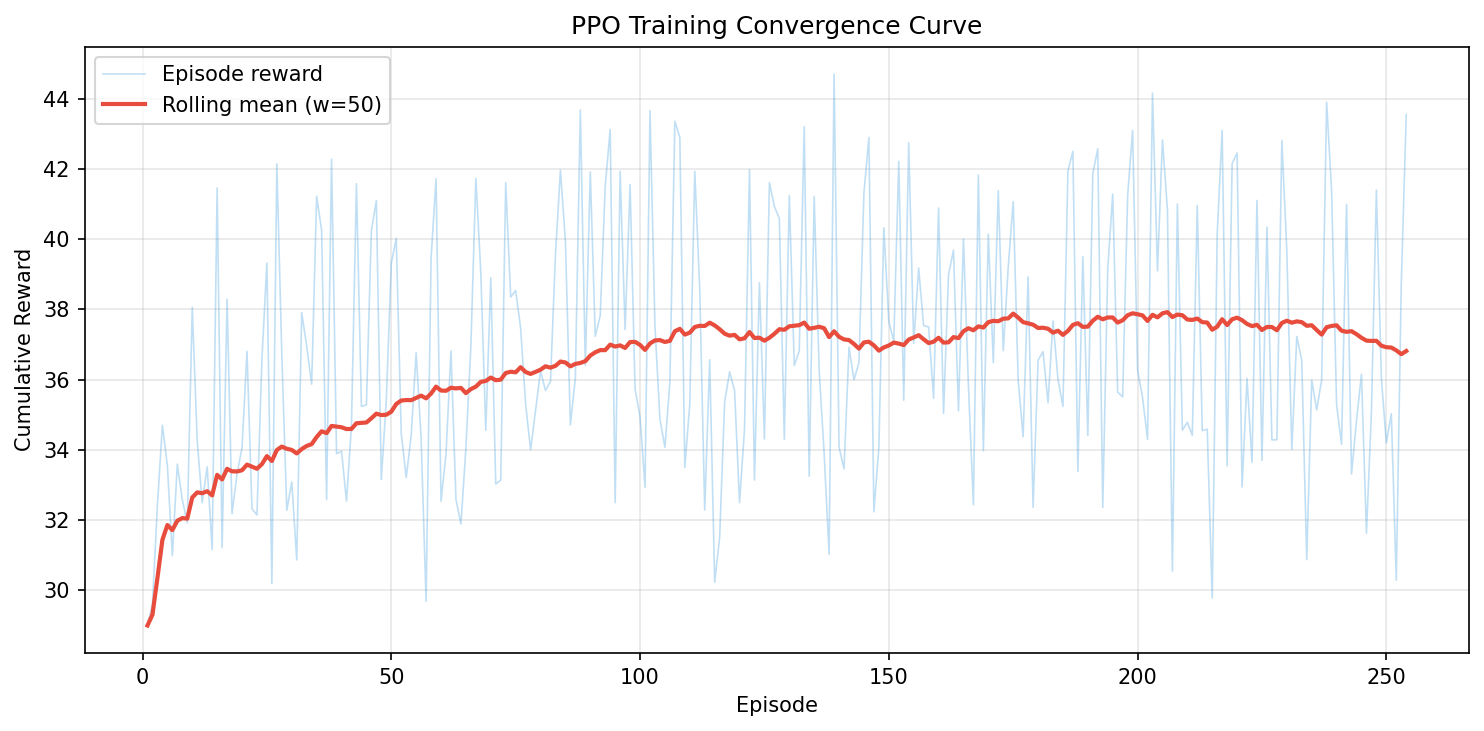
\includegraphics[width=0.85\textwidth]{figures/ppo_training_curve.png}
    \caption{PPO training curve: episode reward versus training episode. The
    shaded region indicates $\pm 1$ standard deviation computed over a
    rolling window. Training was performed with seed 42, learning rate
    $3 \times 10^{-4}$, 1\,024 rollout steps, batch size 64, and 10 PPO
    epochs per update.}
    \label{fig:ppo-appendix}
\end{figure}

